\section{Implementación}

Con la data limpiada, ahora podemos implementar nuestro modelo planteado.

\subsection{Frecuencia}

La implementación del modelado de frecuencia se desarrolló siguiendo la metodología establecida en la sección de modelación, utilizando los estimadores implementados en \texttt{src/utils/Estimadores\_frecuencia.R}. El proceso se ejecutó en el notebook \texttt{modelo\_de\_frecuencia.ipynb} con los siguientes resultados por cobertura:

\subsubsection{Análisis de frecuencia histórica por cobertura}

\textbf{Cobertura PPD (Pérdida Parcial por Daños):}
\begin{itemize}
    \item \textbf{Datos observados:} $N = 365$ días, $\bar{x} = 41.1973$, $\text{Var} = 54.3291$
    \item \textbf{Índice de sobredispersión:} $\frac{\text{Var}}{\bar{x}} = 1.3188 > 1$ (sobredispersión evidente)
    \item \textbf{Distribución seleccionada:} Binomial Negativa (AIC = 2495.61) vs Poisson (AIC = 2508.72)
    \item \textbf{Parámetros estimados:} $\text{size} = 129.2444$, $\mu = 41.1973$
    \item \textbf{Pruebas de bondad:} Chi-cuadrado para Poisson ($\chi^2, p = 0.0798$) y Binomial Negativa ($\chi^2, p = 0.2293$) muestran buen ajuste ($p > 0.05$), pero la prueba Cameron-Trivedi confirma sobredispersión significativa ($z = 3.2161, p = 0.0006$)
\end{itemize}

\textbf{Cobertura PPH (Pérdida Parcial por Hurto):}
\begin{itemize}
    \item \textbf{Datos observados:} $N = 300$ días, $\bar{x} = 2.0967$, $\text{Var} = 1.2782$
    \item \textbf{Índice de sobredispersión:} $\frac{\text{Var}}{\bar{x}} = 0.6097 < 1$ (subdispersión)
    \item \textbf{Distribución seleccionada:} Poisson (AIC = 933.08) vs Binomial Negativa (AIC = 935.95)
    \item \textbf{Parámetros estimados:} $\lambda = 2.0967$
    \item \textbf{Pruebas de bondad:} Chi-cuadrado para ambas distribuciones muestra mal ajuste ($p = 0.0025$), pero Cameron-Trivedi confirma ausencia de sobredispersión ($z = -7.4502, p = 1.0000$)
\end{itemize}

\textbf{Cobertura PTH (Pérdida Total por Hurto):}
\begin{itemize}
    \item \textbf{Datos observados:} $N = 259$ días, $\bar{x} = 1.9189$, $\text{Var} = 1.0748$
    \item \textbf{Índice de sobredispersión:} $\frac{\text{Var}}{\bar{x}} = 0.5601 < 1$ (subdispersión)
    \item \textbf{Distribución seleccionada:} Poisson (AIC = 771.79) vs Binomial Negativa (AIC = 774.52)
    \item \textbf{Parámetros estimados:} $\lambda = 1.9189$
    \item \textbf{Pruebas de bondad:} Chi-cuadrado para ambas distribuciones muestra mal ajuste ($p = 0.0007$), pero Cameron-Trivedi confirma ausencia de sobredispersión ($z = -7.9778, p = 1.0000$)
\end{itemize}

\textbf{Cobertura RC (Responsabilidad Civil):}
\begin{itemize}
    \item \textbf{Datos observados:} $N = 365$ días, $\bar{x} = 7.8849$, $\text{Var} = 9.8494$
    \item \textbf{Índice de sobredispersión:} $\frac{\text{Var}}{\bar{x}} = 1.2491 > 1$ (sobredispersión evidente)
    \item \textbf{Distribución seleccionada:} Binomial Negativa (AIC = 1858.58) vs Poisson (AIC = 1866.02)
    \item \textbf{Parámetros estimados:} $\text{size} = 31.6513$, $\mu = 7.8849$
    \item \textbf{Pruebas de bondad:} Chi-cuadrado para Poisson ($\chi^2, p = 0.1991$) y Binomial Negativa ($\chi^2, p = 0.6595$) muestran buen ajuste, y Cameron-Trivedi confirma sobredispersión ($z = 2.7632, p = 0.0029$)
\end{itemize}

\subsubsection{Metodología de pruebas estadísticas}

Para determinar la mejor distribución entre Poisson y Binomial Negativa se implementaron múltiples criterios estadísticos:

\begin{itemize}
    \item \textbf{Criterio de Información de Akaike (AIC):} Para selección de modelo con penalización por complejidad
    \item \textbf{Prueba Chi-cuadrado de bondad de ajuste:} Comparando frecuencias observadas vs esperadas bajo cada distribución
    \item \textbf{Prueba Cameron-Trivedi:} Test específico de sobredispersión basado en regresión GLM Poisson
    \item \textbf{Índice de dispersión:} Ratio varianza/media como indicador de sobredispersión
\end{itemize}

La prueba Cameron-Trivedi es particularmente relevante pues evalúa directamente si los datos presentan sobredispersión significativa que justifique el uso de Binomial Negativa sobre Poisson. Esta prueba utiliza un modelo GLM Poisson auxiliar y evalúa si la varianza condicional excede la media bajo la hipótesis nula de equidispersión.

\subsubsection{Cálculo de intensidades de siniestralidad}

Para cada cobertura se calculó la intensidad $\lambda_c$ como el cociente entre la frecuencia promedio de siniestros y el número promedio de pólizas vigentes:

\begin{align}
\lambda_{PPD} &= 0.0002240547\\
\lambda_{PPH} &= 1.141035 \times 10^{-5}\\
\lambda_{PTH} &= 1.037491 \times 10^{-5}\\
\lambda_{RC} &= 5.189072 \times 10^{-5}
\end{align}

\subsubsection{Modelado para el nuevo portafolio}

Aplicando las intensidades calculadas al nuevo portafolio y manteniendo los índices de sobredispersión, se obtuvieron las siguientes distribuciones de frecuencia:

\begin{align}
N^{(PPD)} &\sim \text{BinNeg}(r = 0.00419, p = 0.758)\\
N^{(PPH)} &\sim \text{Poisson}(\lambda = 0.00134)\\
N^{(PTH)} &\sim \text{Poisson}(\lambda = 0.00122)\\
N^{(RC)} &\sim \text{BinNeg}(r = 0.01863, p = 0.800)
\end{align}

\subsection{Severidad}

La implementación del modelado de severidad se desarrolló en el notebook \texttt{modelo\_de\_severidad.ipynb} siguiendo un proceso sistemático de análisis exploratorio, limpieza de datos y ajuste de distribuciones.

\subsubsection{Análisis inicial de datos originales}

Al cargar los datos de severidad por cobertura desde los archivos procesados, se observó inmediatamente que las distribuciones presentaban serios problemas de calidad. Los datos originales mostraron distribuciones extremadamente sesgadas con presencia masiva de outliers que impedirían cualquier ajuste distribucional adecuado.

\begin{figure}[H]
    \centering
    \begin{subfigure}{0.35\textwidth}
        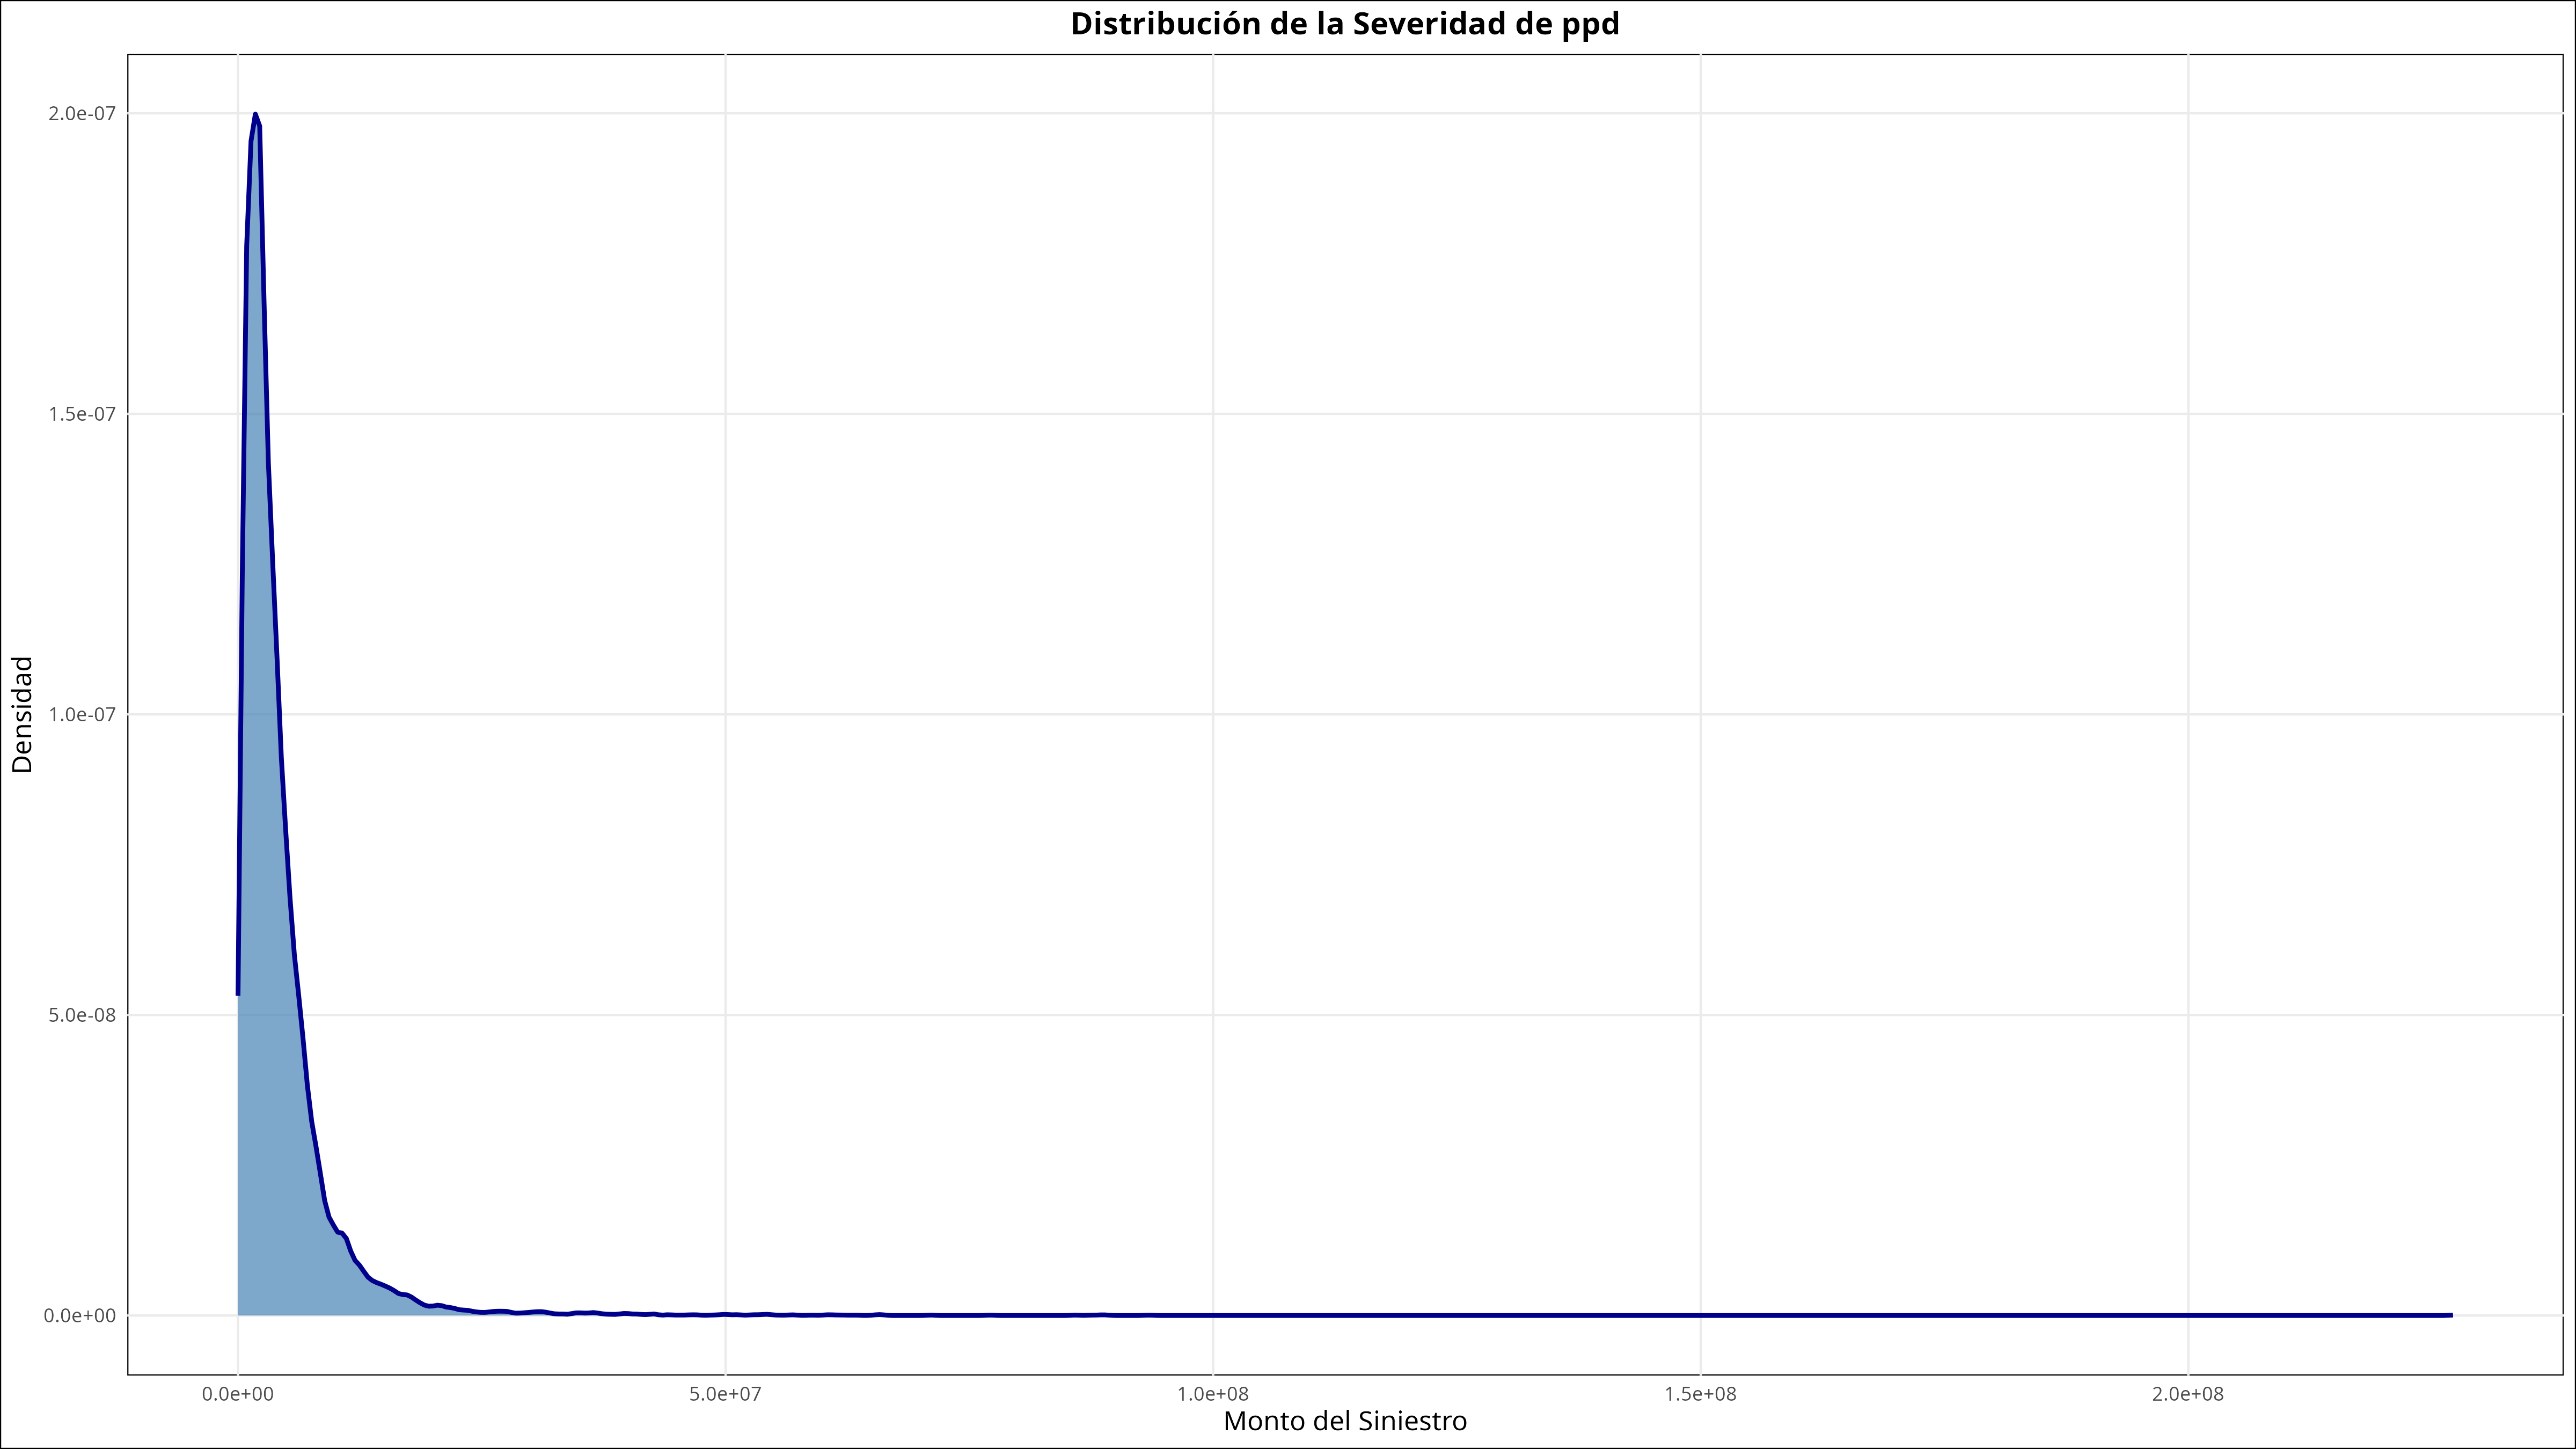
\includegraphics[width=\textwidth]{../images/distribucion_severidad_ppd.png}
        \caption{Severidad PPD original}
    \end{subfigure}
    \hfill
    \begin{subfigure}{0.35\textwidth}
        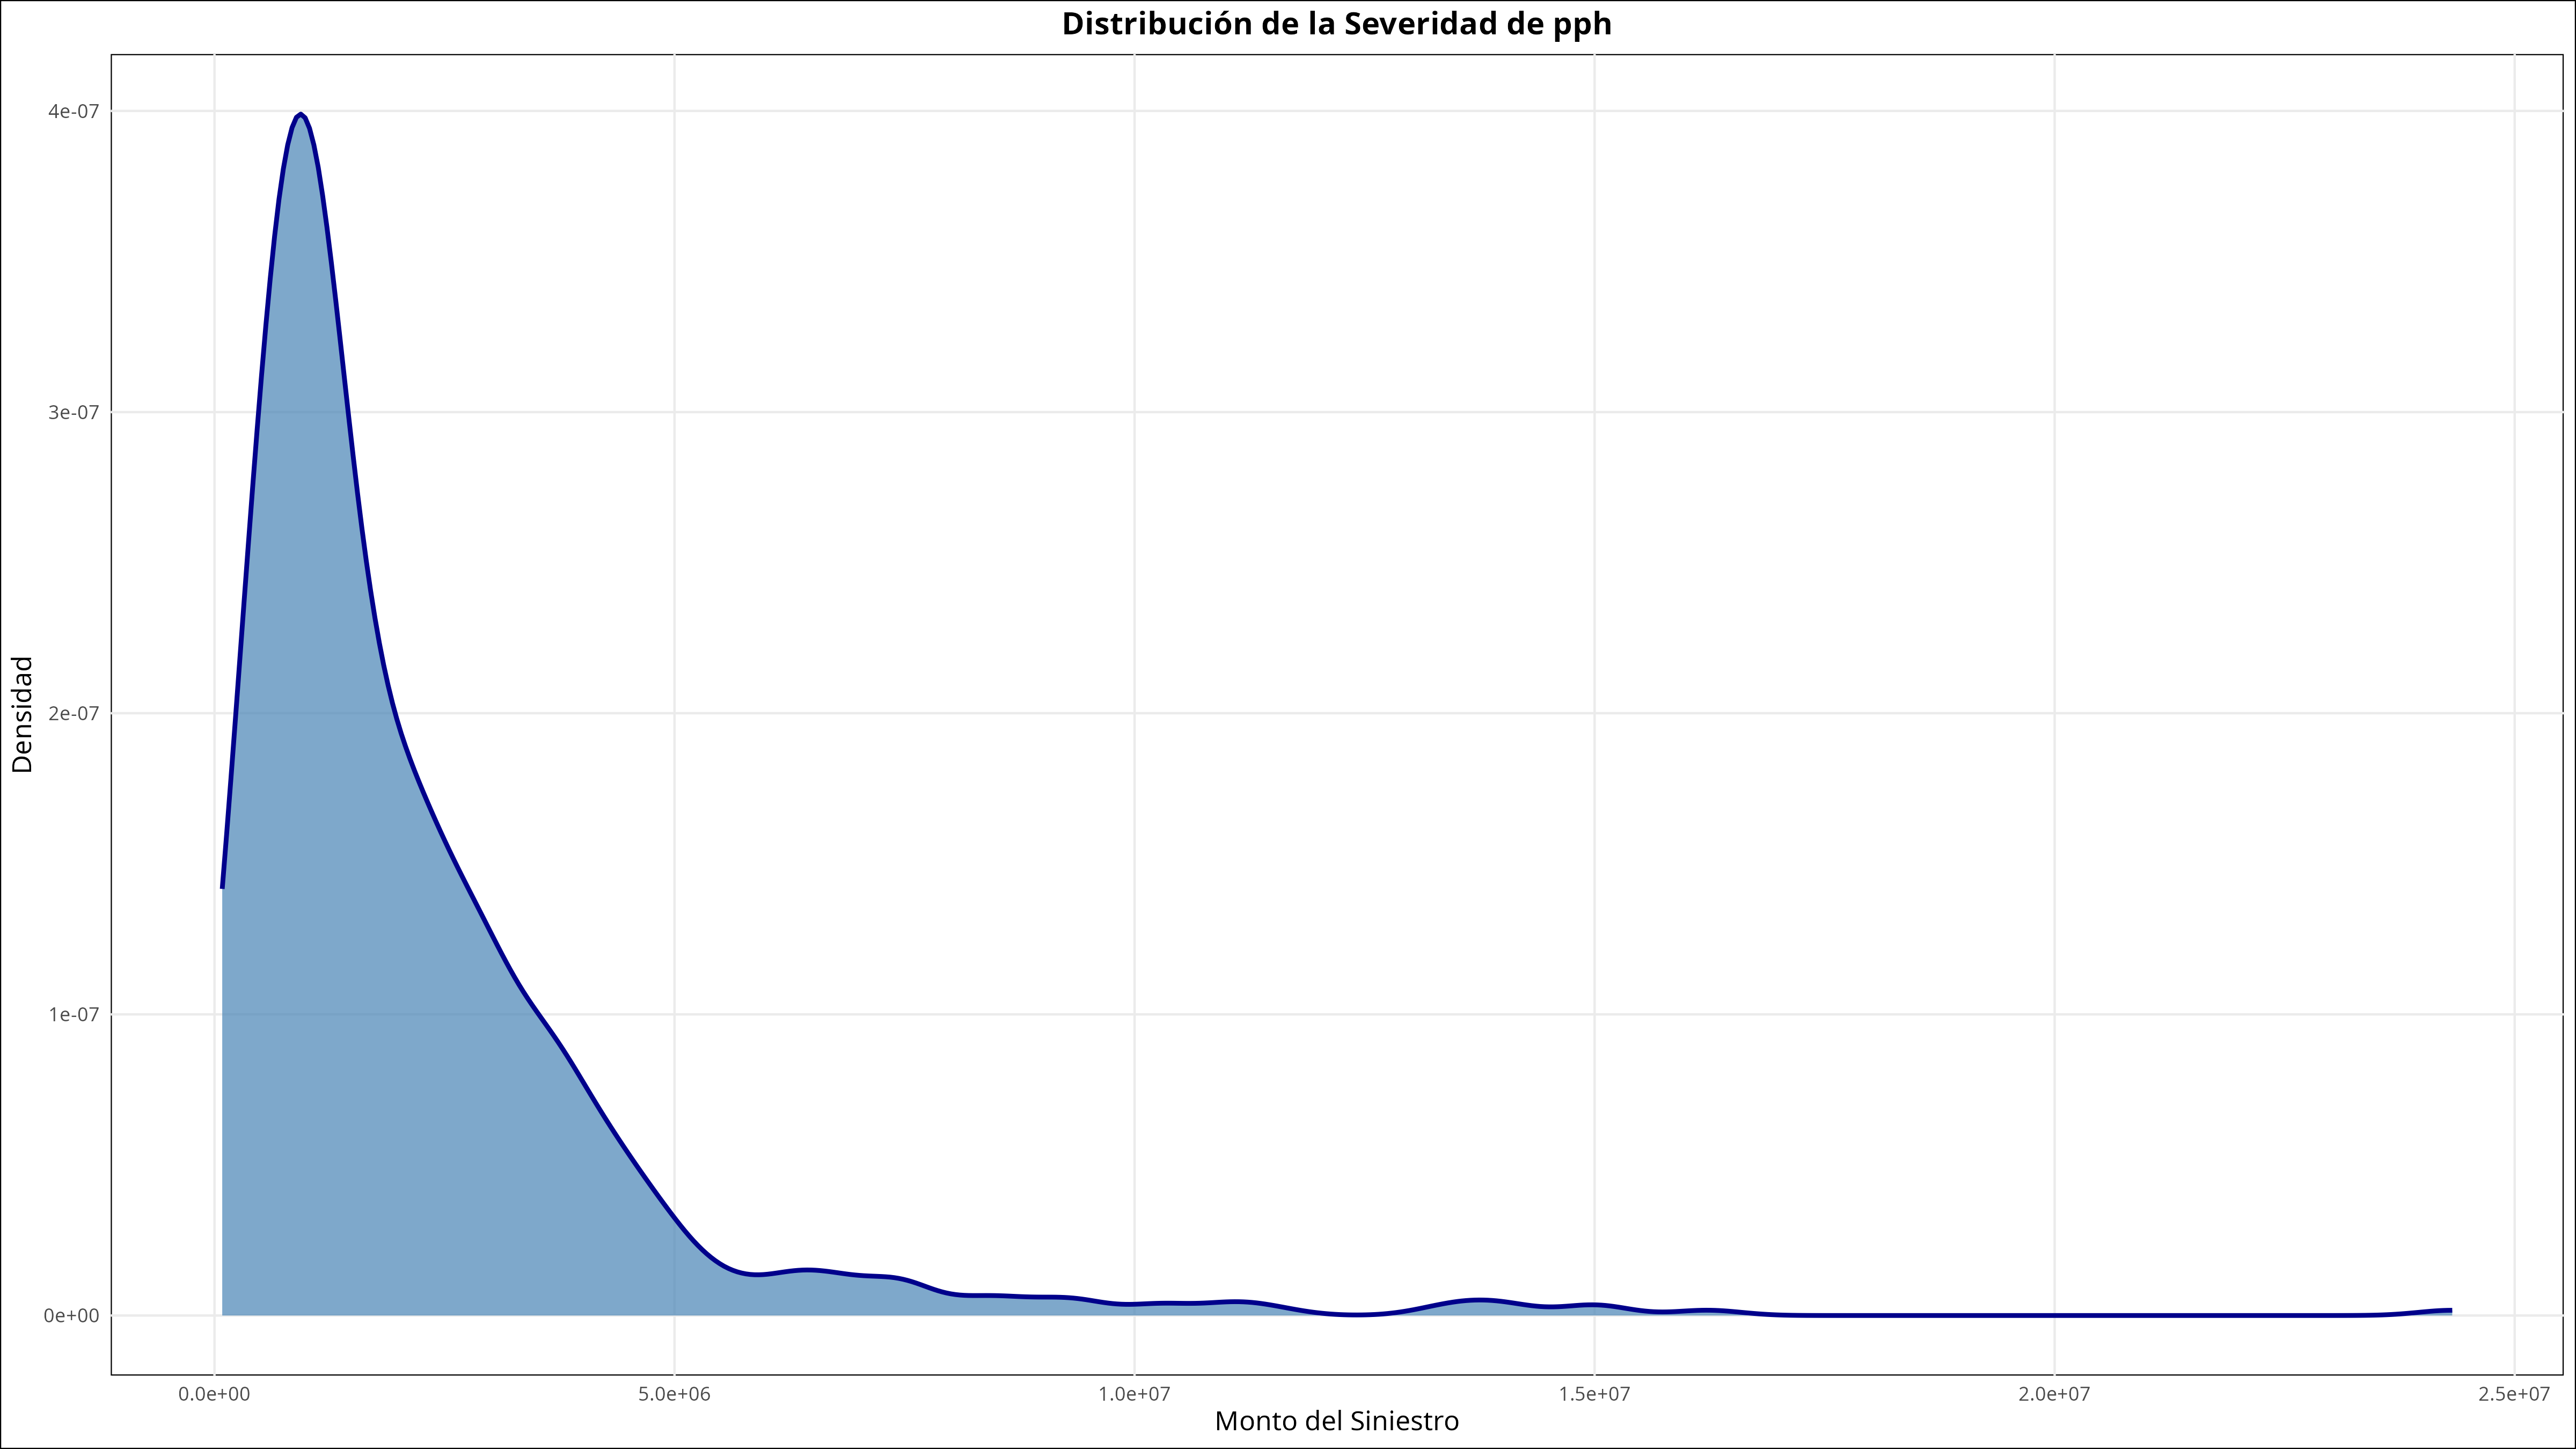
\includegraphics[width=\textwidth]{../images/distribucion_severidad_pph.png}
        \caption{Severidad PPH original}
    \end{subfigure}
    \\[0.5em]
    \begin{subfigure}{0.35\textwidth}
        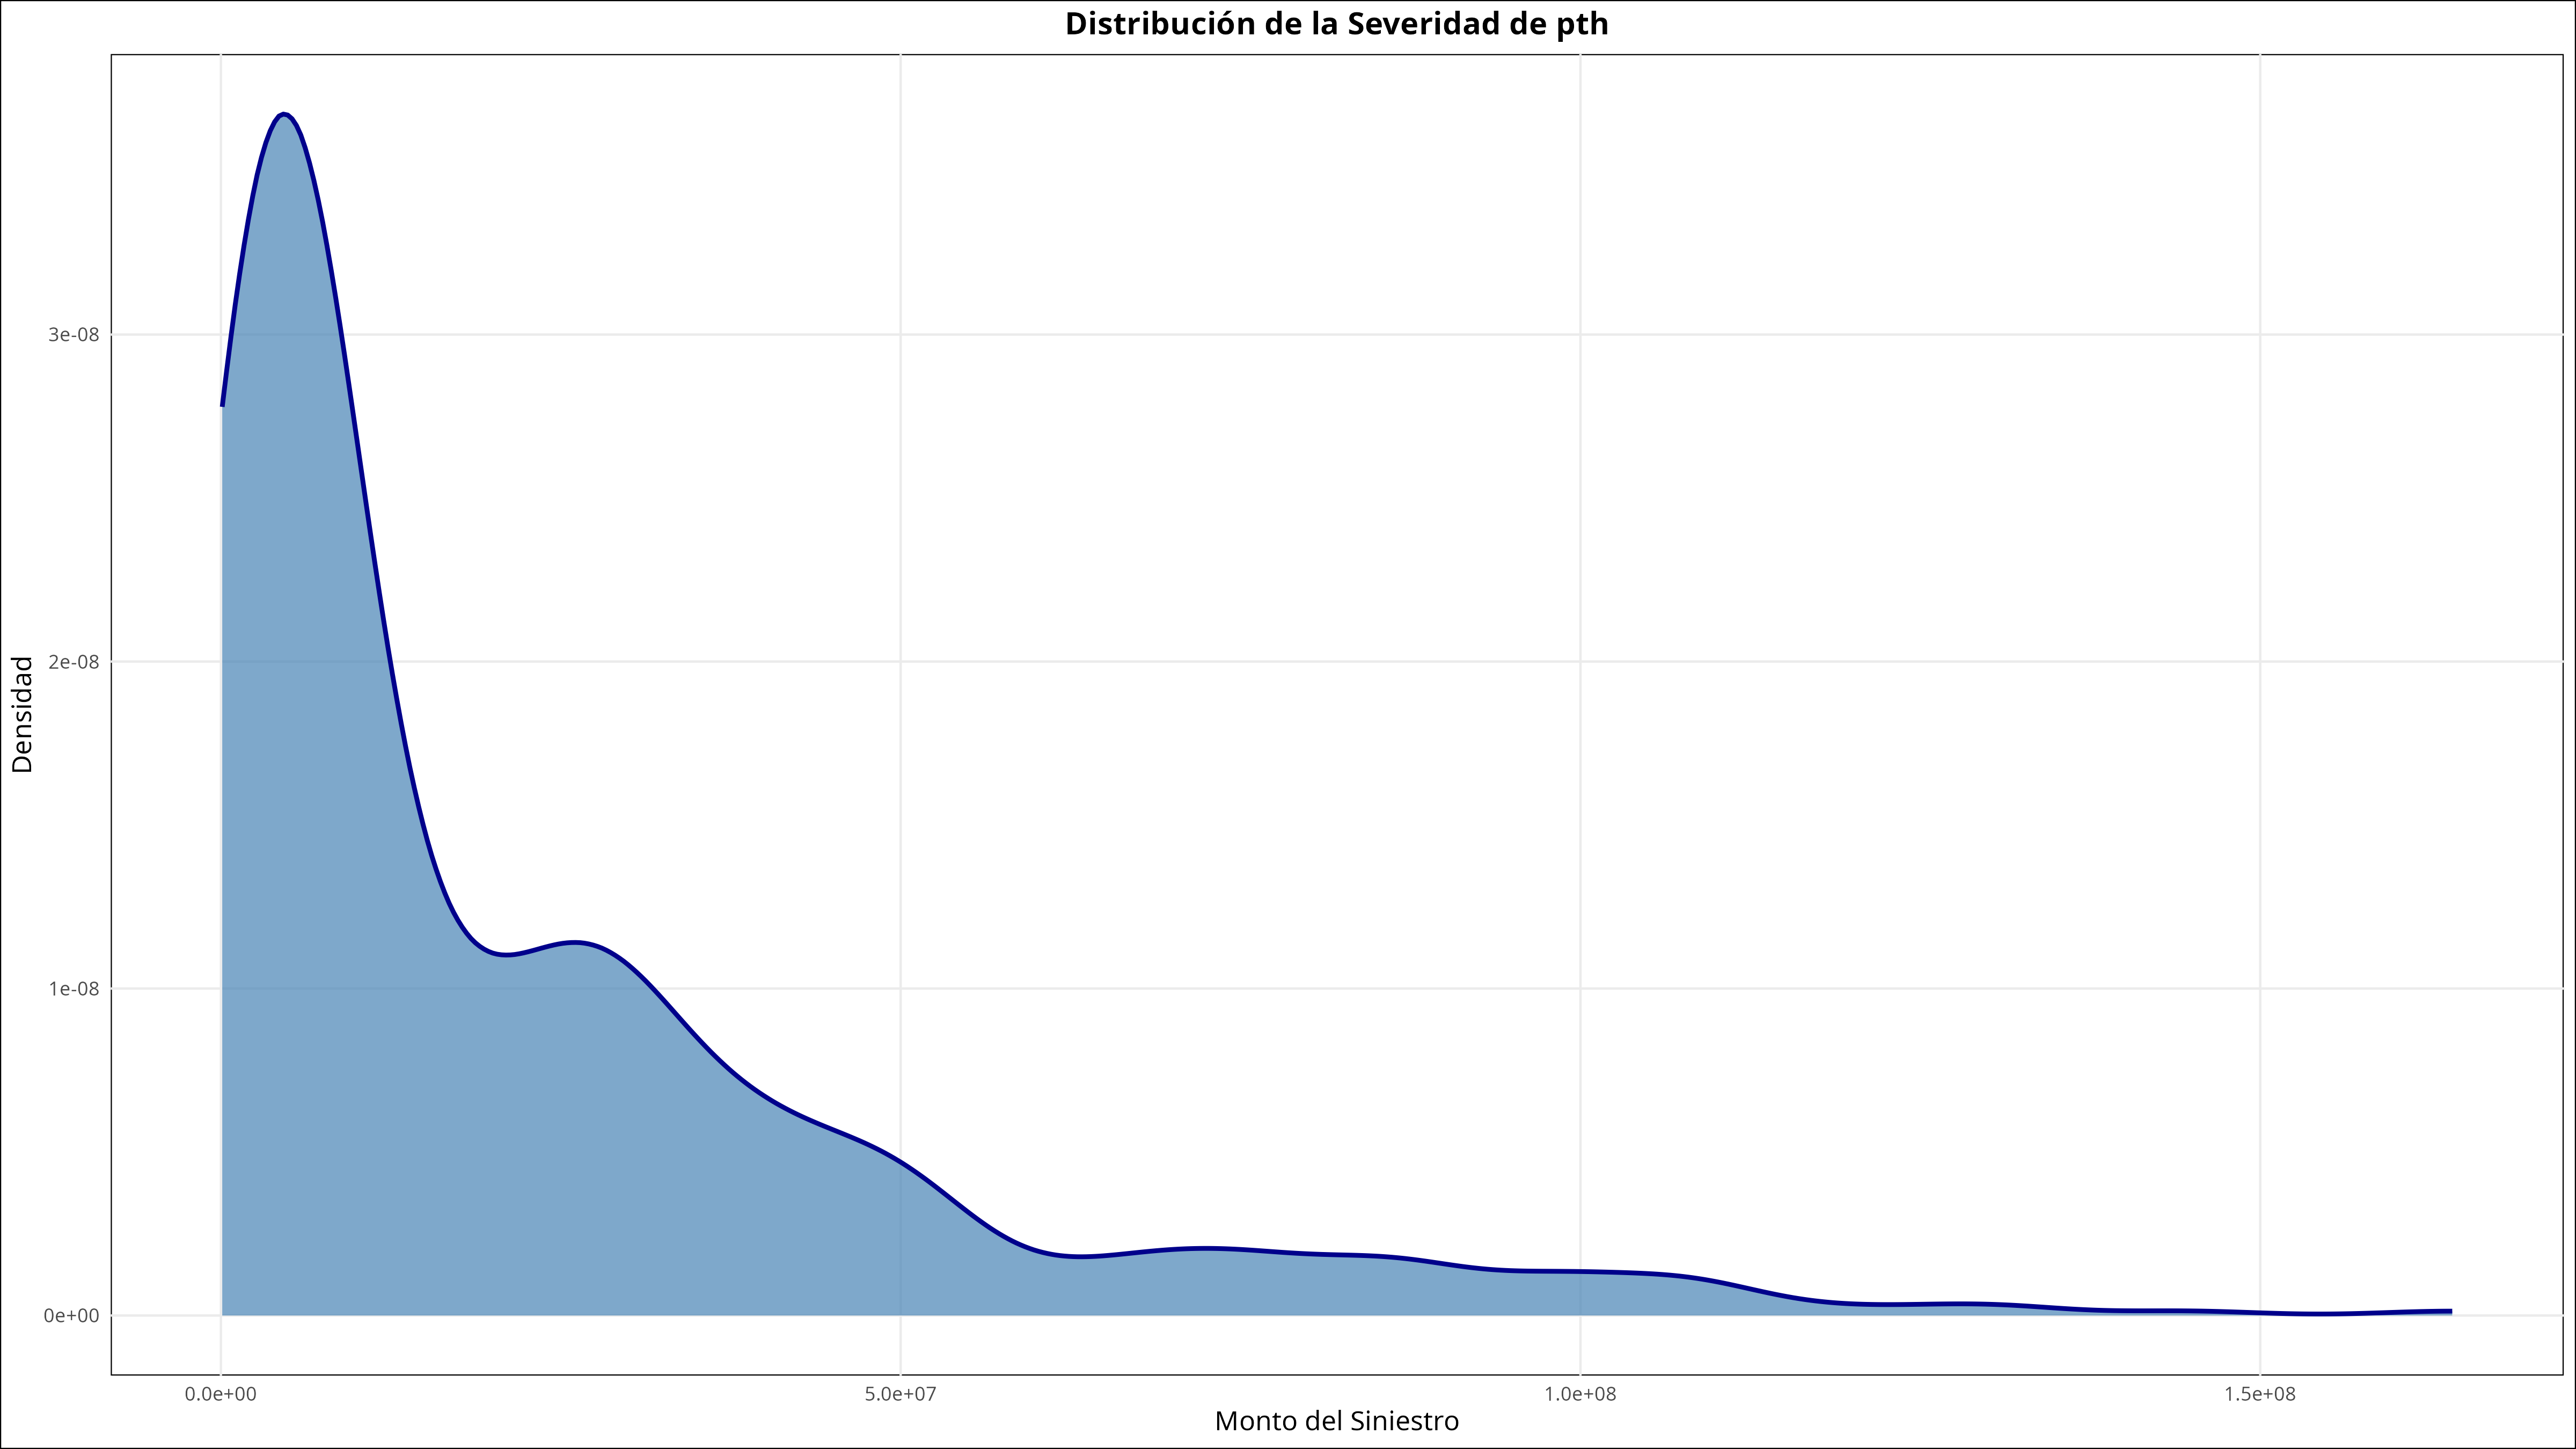
\includegraphics[width=\textwidth]{../images/distribucion_severidad_pth.png}
        \caption{Severidad PTH original}
    \end{subfigure}
    \hfill
    \begin{subfigure}{0.35\textwidth}
        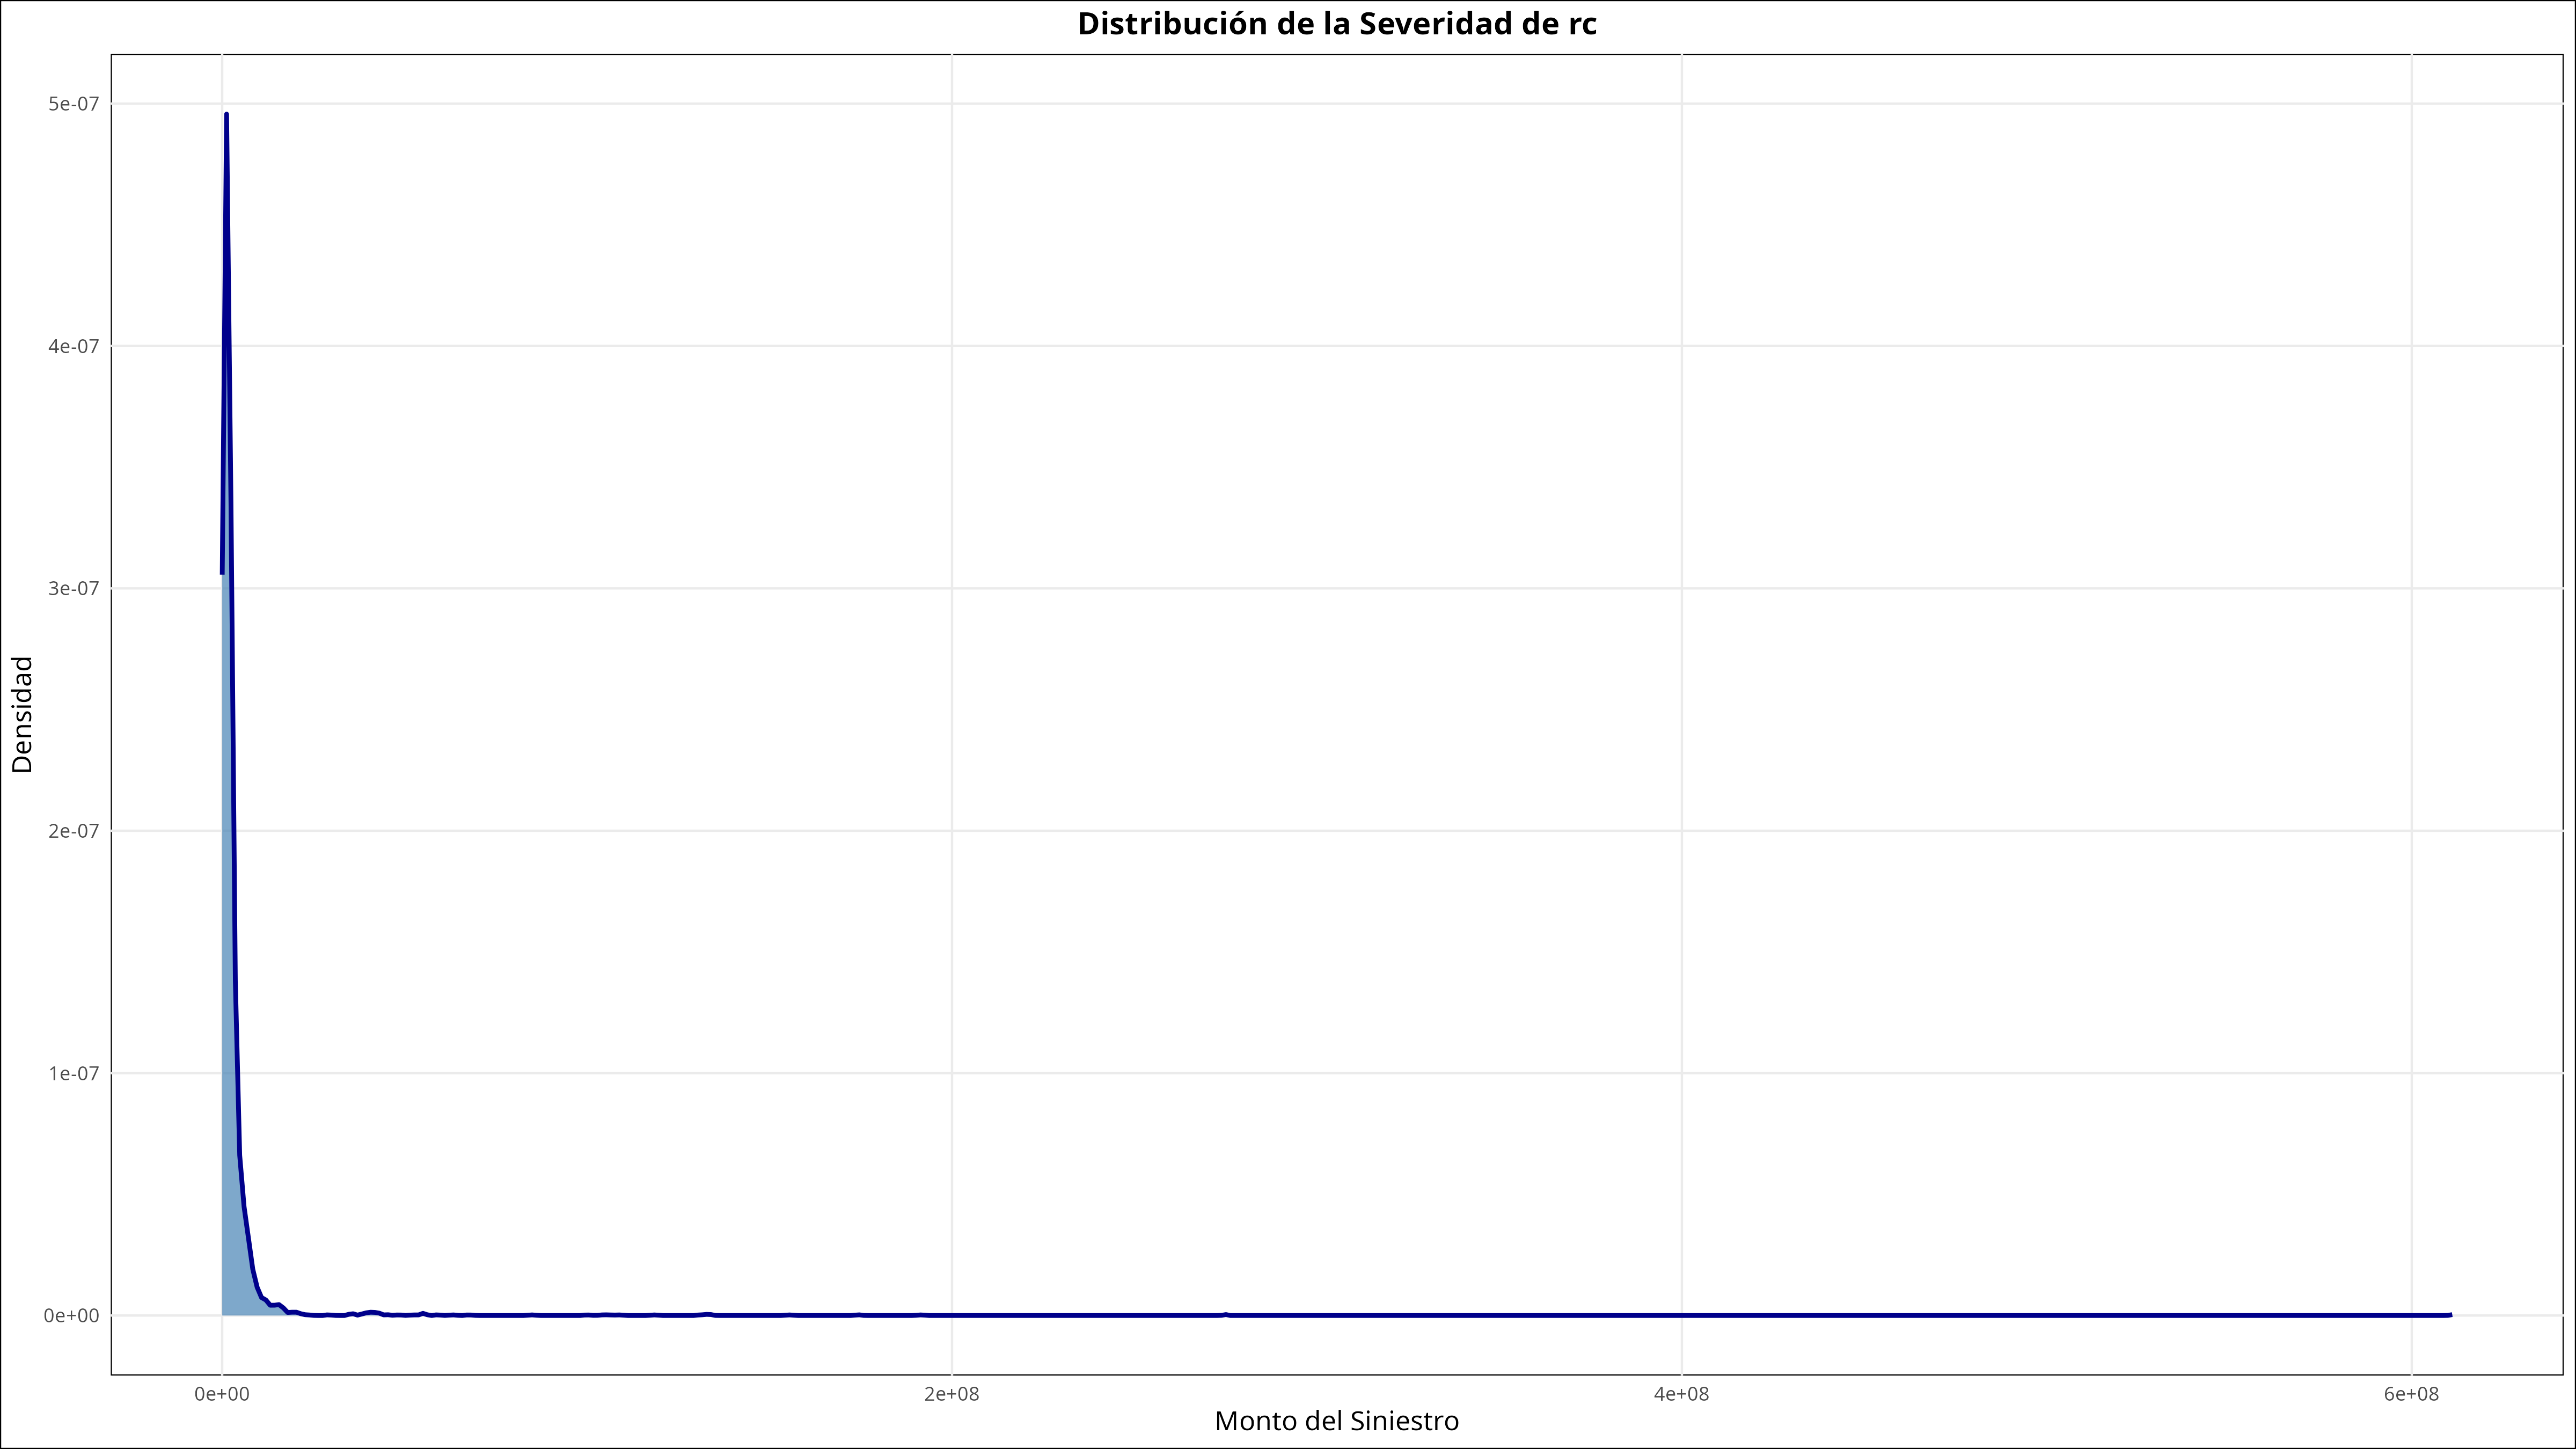
\includegraphics[width=\textwidth]{../images/distribucion_severidad_rc.png}
        \caption{Severidad RC original}
    \end{subfigure}
\end{figure}

Como se evidencia en la Figura \ref{fig:severidad_original}, todas las coberturas presentaron distribuciones con colas extremadamente pesadas y concentración excesiva en valores atípicos, haciendo necesario un proceso de filtrado robusto antes de cualquier intento de modelación.

\subsubsection{Filtrado de outliers con Z-score robusto}

Para abordar la presencia masiva de outliers, se implementó el algoritmo de detección basado en Z-score robusto disponible en \texttt{src/utils/Excluir\_outliers.R}. Este método utiliza estadísticos resistentes que no se ven afectados por valores extremos:

El algoritmo calcula Z-scores robustos mediante:
\begin{equation*}
z_i = \frac{|x_i - \text{mediana}|}{\text{MAD}}
\end{equation*}

donde MAD es la desviación absoluta mediana, definida como:
\begin{equation*}
\text{MAD} = \text{mediana}(|x_i - \text{mediana}(x)|)
\end{equation*}

Se aplicaron diferentes umbrales según las características específicas de cada cobertura:
\begin{itemize}
    \item \textbf{PPD:} Umbral $= 20$ (datos con alta variabilidad natural)
    \item \textbf{PPH:} Umbral $= 15$ (outliers moderados)  
    \item \textbf{PTH:} Umbral $= 10$ (concentración de valores extremos)
    \item \textbf{RC:} Umbral $= 20$ (similar dispersión a PPD)
\end{itemize}

\subsubsection{Ajuste de distribuciones con fitdistr()}

Una vez filtrados los outliers, se procedió al ajuste sistemático de múltiples familias de distribuciones utilizando la función \texttt{fitdistr()} del paquete MASS de R. Se evaluaron las siguientes distribuciones por máxima verosimilitud:

\begin{itemize}
    \item \textbf{Normal:} $f(x) = \frac{1}{\sigma\sqrt{2\pi}} e^{-\frac{(x-\mu)^2}{2\sigma^2}}$
    \item \textbf{Lognormal:} $f(x) = \frac{1}{x\sigma\sqrt{2\pi}} e^{-\frac{(\ln x-\mu)^2}{2\sigma^2}}$
    \item \textbf{Gamma:} $f(x) = \frac{\beta^\alpha}{\Gamma(\alpha)} x^{\alpha-1} e^{-\beta x}$
    \item \textbf{Weibull:} $f(x) = \frac{k}{\lambda}\left(\frac{x}{\lambda}\right)^{k-1} e^{-(x/\lambda)^k}$
    \item \textbf{Pareto:} $f(x) = \frac{\alpha \theta^\alpha}{x^{\alpha+1}}$ para $x \geq \theta$
\end{itemize}

Durante el proceso de ajuste, se observó que las distribuciones Gamma y Pareto fallaron sistemáticamente por problemas de convergencia en la optimización numérica, debido a las características particulares de los datos de seguros que no se adaptan bien a estas familias distribucionales.

\subsubsection{Pruebas de bondad de ajuste}

Para evaluar la calidad de los ajustes obtenidos se implementaron múltiples criterios estadísticos:

\begin{itemize}
    \item \textbf{Kolmogorov-Smirnov:} Prueba no paramétrica que compara la función de distribución empírica con la teórica, calculando la máxima diferencia absoluta entre ambas
    \item \textbf{Anderson-Darling:} Aplicada específicamente para la distribución Normal, esta prueba es más potente que K-S para detectar diferencias en las colas
    \item \textbf{Criterio de Información de Akaike (AIC):} Para selección de modelo con penalización por complejidad
    \item \textbf{Criterio Bayesiano de Información (BIC):} Criterio más conservador que penaliza más fuertemente la complejidad del modelo
\end{itemize}

Los resultados de ajuste por cobertura fueron:

\textbf{Severidad PPD:} Lognormal (AIC = 485,554.92) vs Normal (AIC = 501,794.68) vs Weibull (AIC = 486,877.20)

\textbf{Severidad PPH:} Lognormal (AIC = 19,509.34) vs Normal (AIC = 20,150.39) vs Weibull (AIC = 19,579.53)

\textbf{Severidad PTH:} Lognormal (AIC = 17,906.02) vs Normal (AIC = 18,453.58)

\textbf{Severidad RC:} Lognormal (AIC = 88,745.03) vs Normal (AIC = 92,260.66) vs Weibull (AIC = 89,532.69)

\subsubsection{Distribuciones seleccionadas}

Todas las coberturas mostraron consistentemente mejor ajuste con distribución Lognormal según todos los criterios estadísticos evaluados:

\begin{align*}
X^{(PPD)} &\sim \text{LogNormal}(\mu = 14.8219, \sigma = 0.9396)\\
X^{(PPH)} &\sim \text{LogNormal}(\mu = 14.2108, \sigma = 0.9048)\\
X^{(PTH)} &\sim \text{LogNormal}(\mu = 16.5134, \sigma = 1.0809)\\
X^{(RC)} &\sim \text{LogNormal}(\mu = 14.4446, \sigma = 0.7865)
\end{align*}

Este resultado es altamente consistente con la literatura actuarial, donde la distribución Lognormal es ampliamente utilizada para modelar severidad de siniestros debido a su capacidad natural para capturar la asimetría positiva característica de los datos de seguros.

\subsubsection{Visualización final de ajustes}

Las gráficas finales muestran los histogramas de los datos filtrados con las densidades Lognormal ajustadas superpuestas, confirmando visualmente la calidad de los ajustes obtenidos.

\begin{figure}[H]
    \centering
    \begin{subfigure}{0.45\textwidth}
        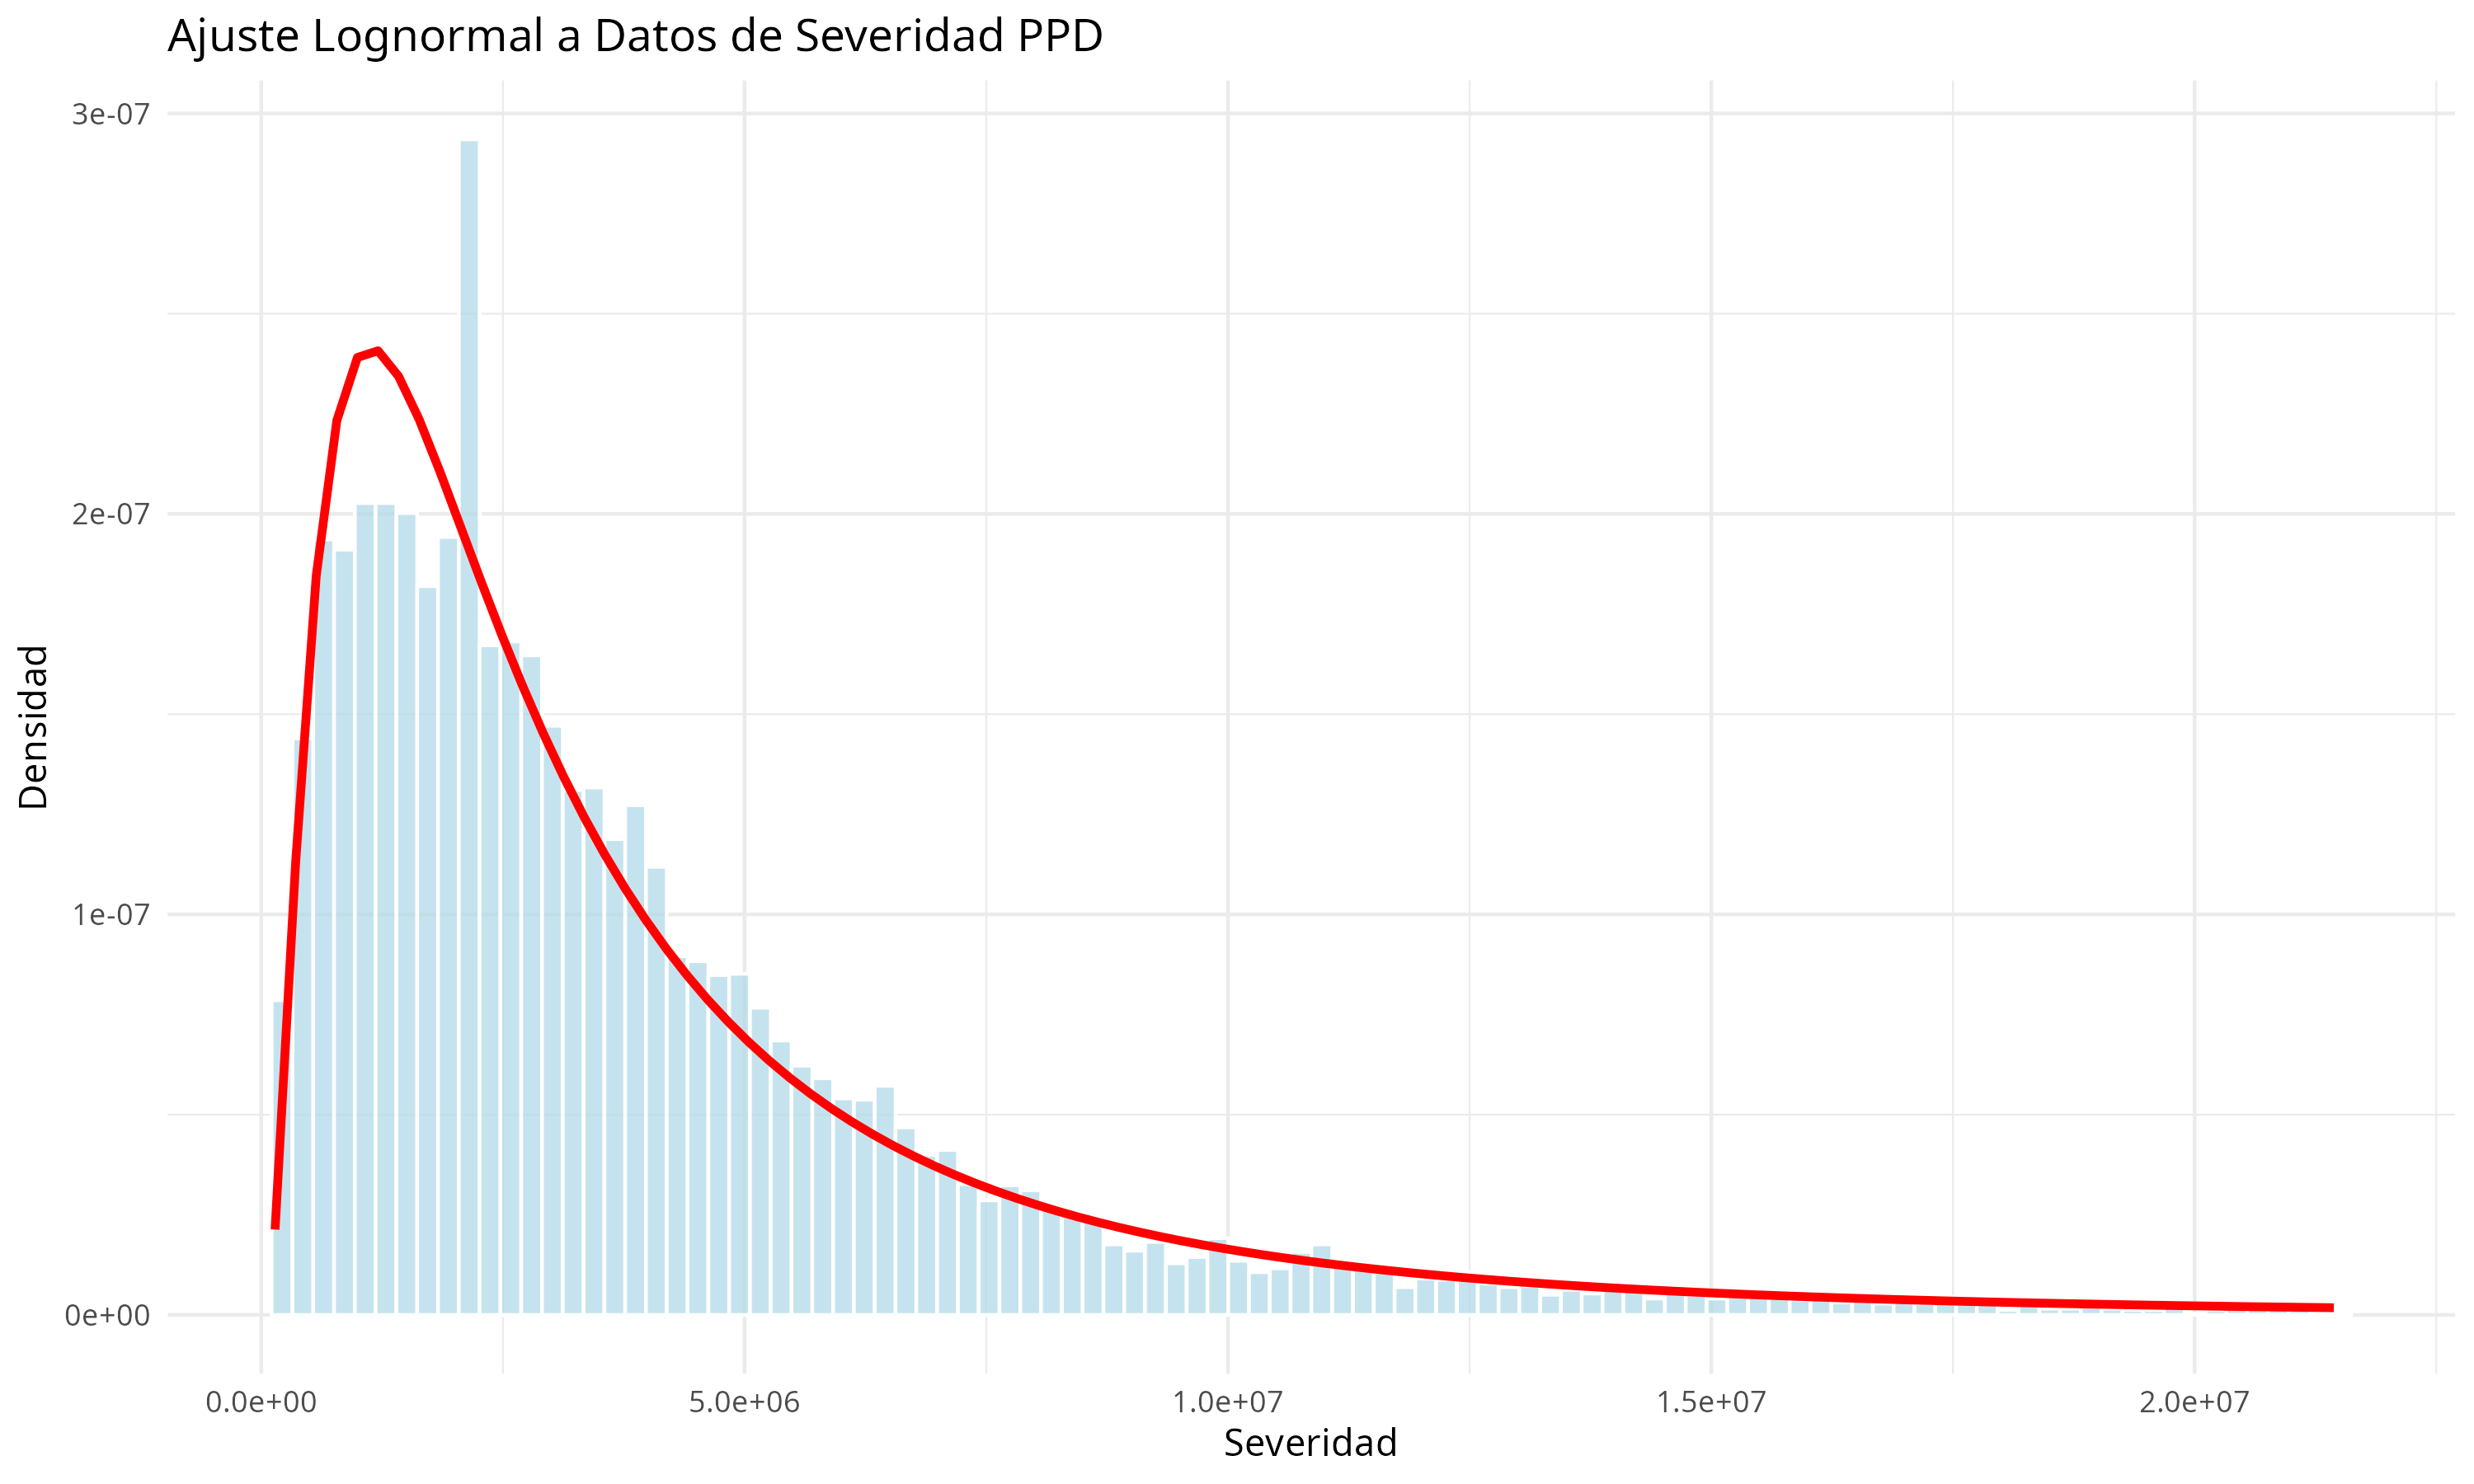
\includegraphics[width=\textwidth]{../images/ajuste_lognormal_ppd.png}
        \caption{Ajuste Lognormal PPD}
    \end{subfigure}
    \hfill
    \begin{subfigure}{0.45\textwidth}
        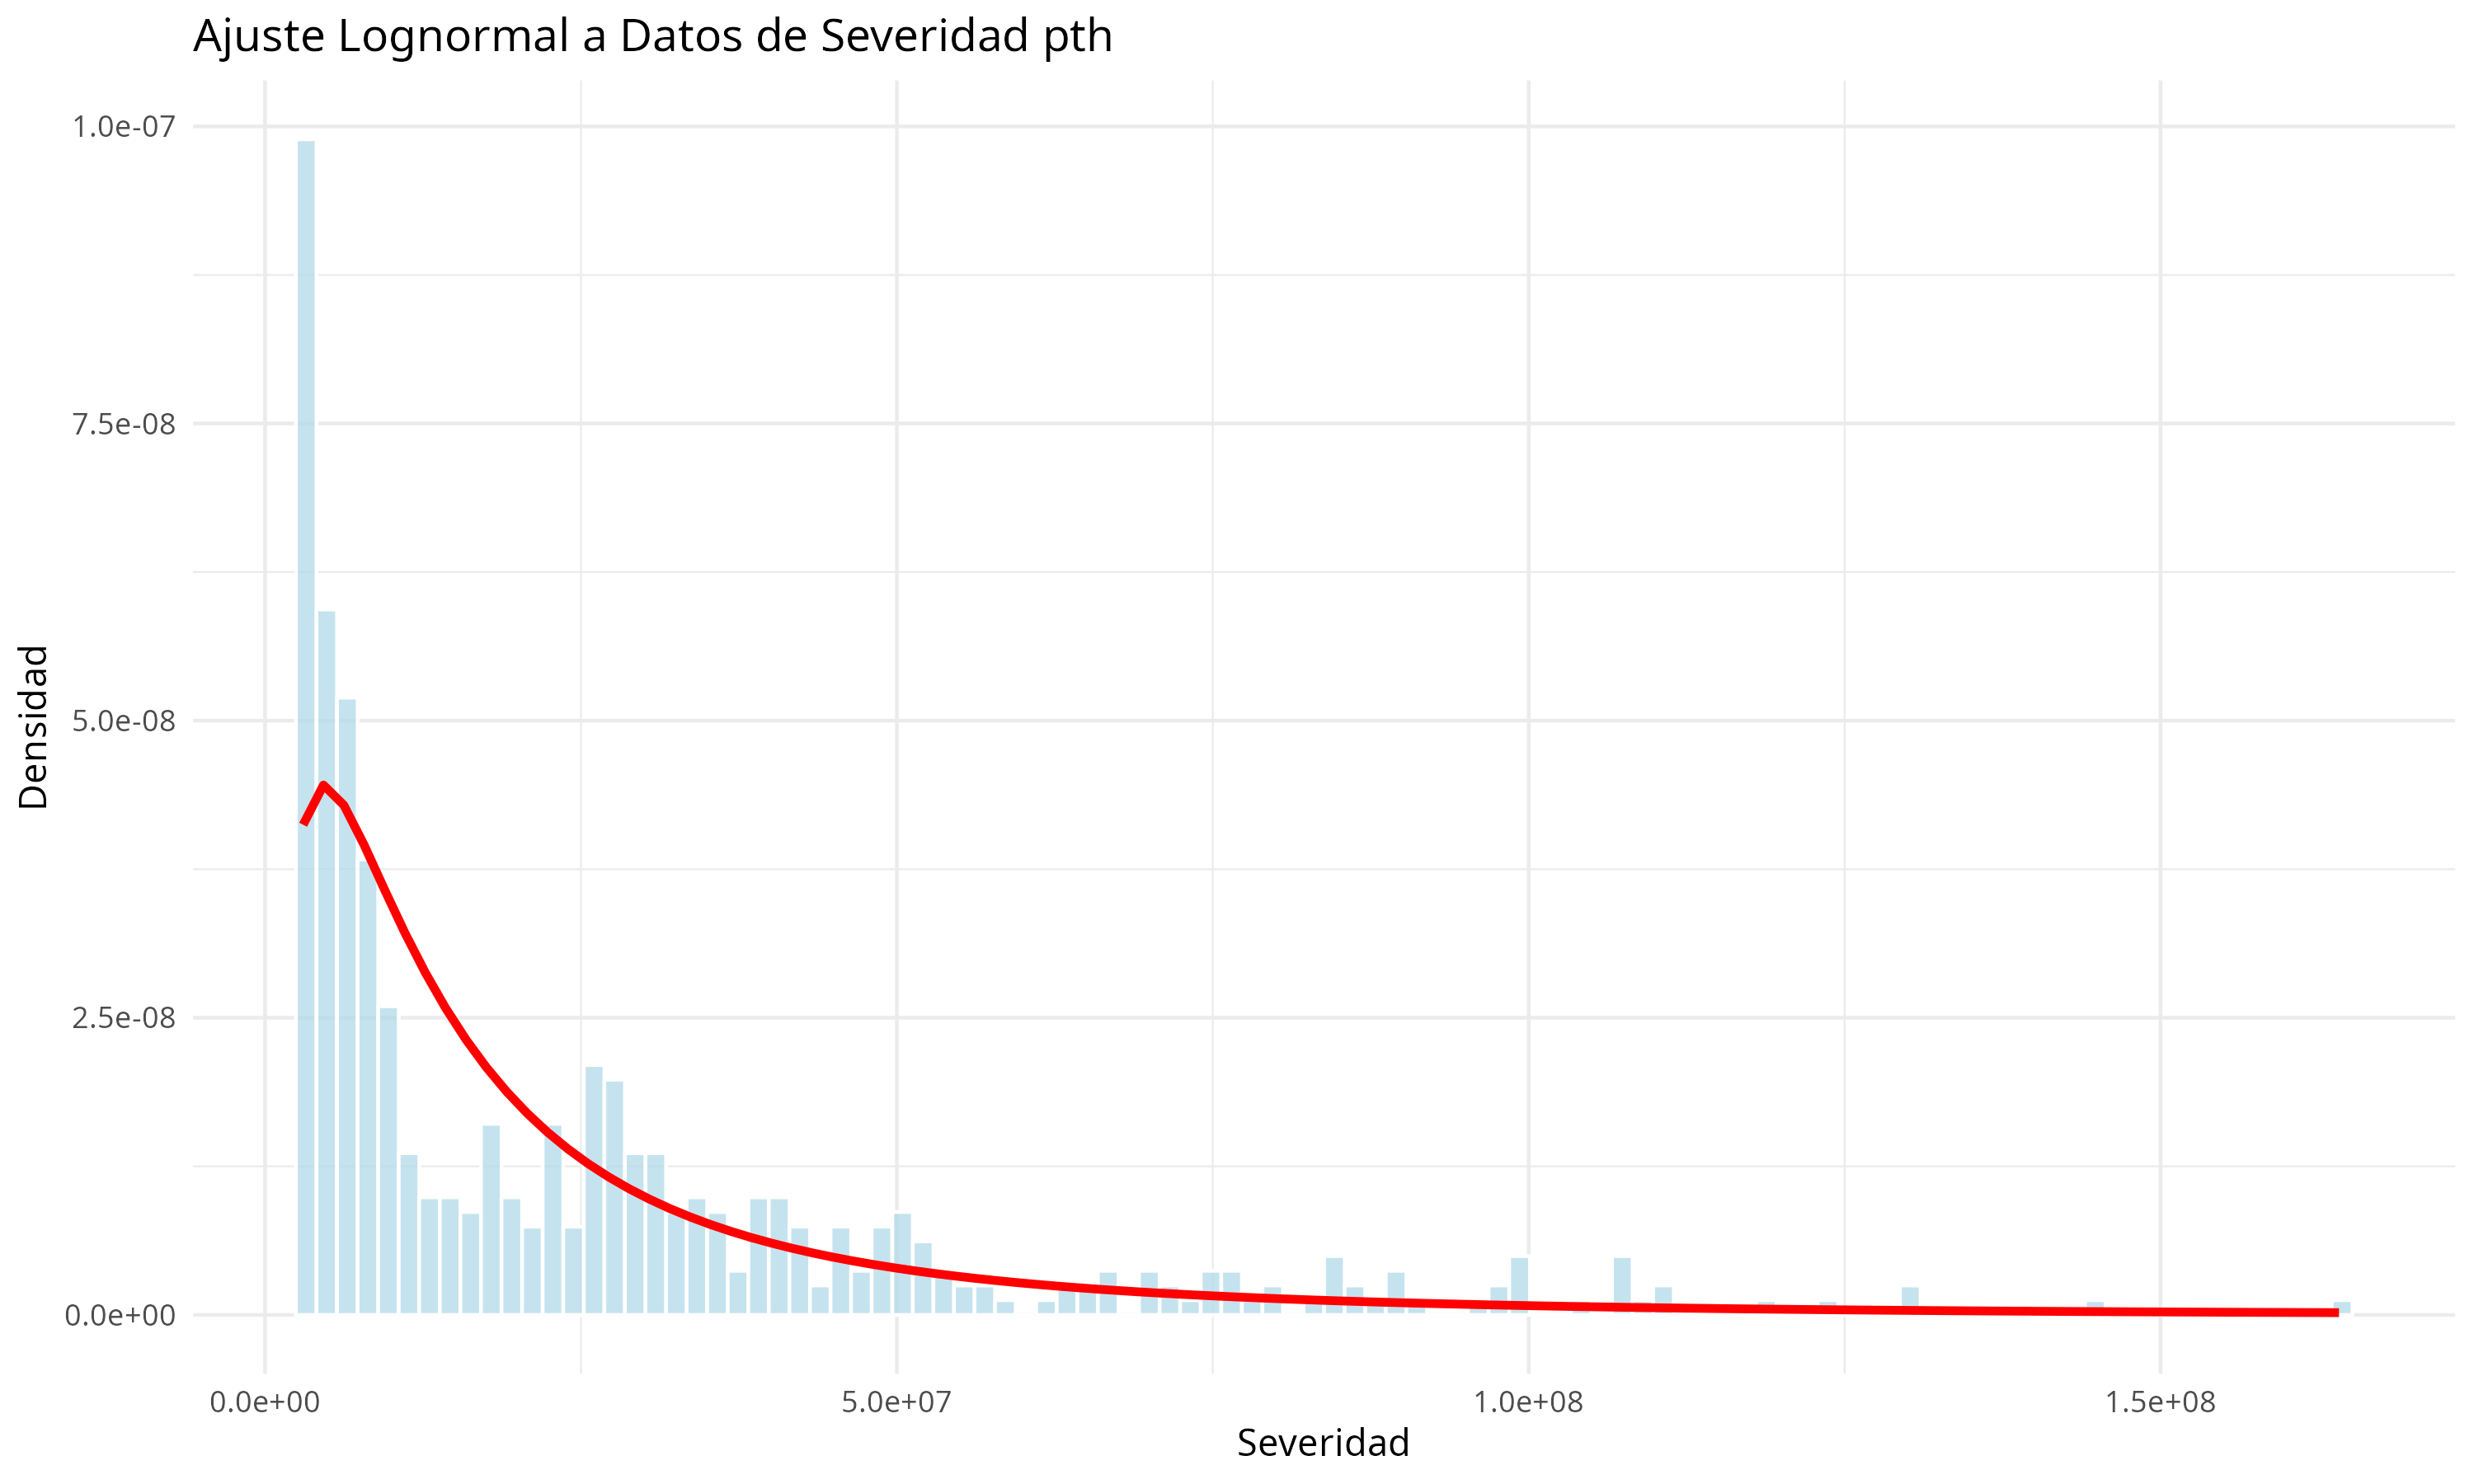
\includegraphics[width=\textwidth]{../images/ajuste_lognormal_pth.png}
        \caption{Ajuste Lognormal PTH}
    \end{subfigure}
    \\[0.5em]
    \begin{subfigure}{0.45\textwidth}
        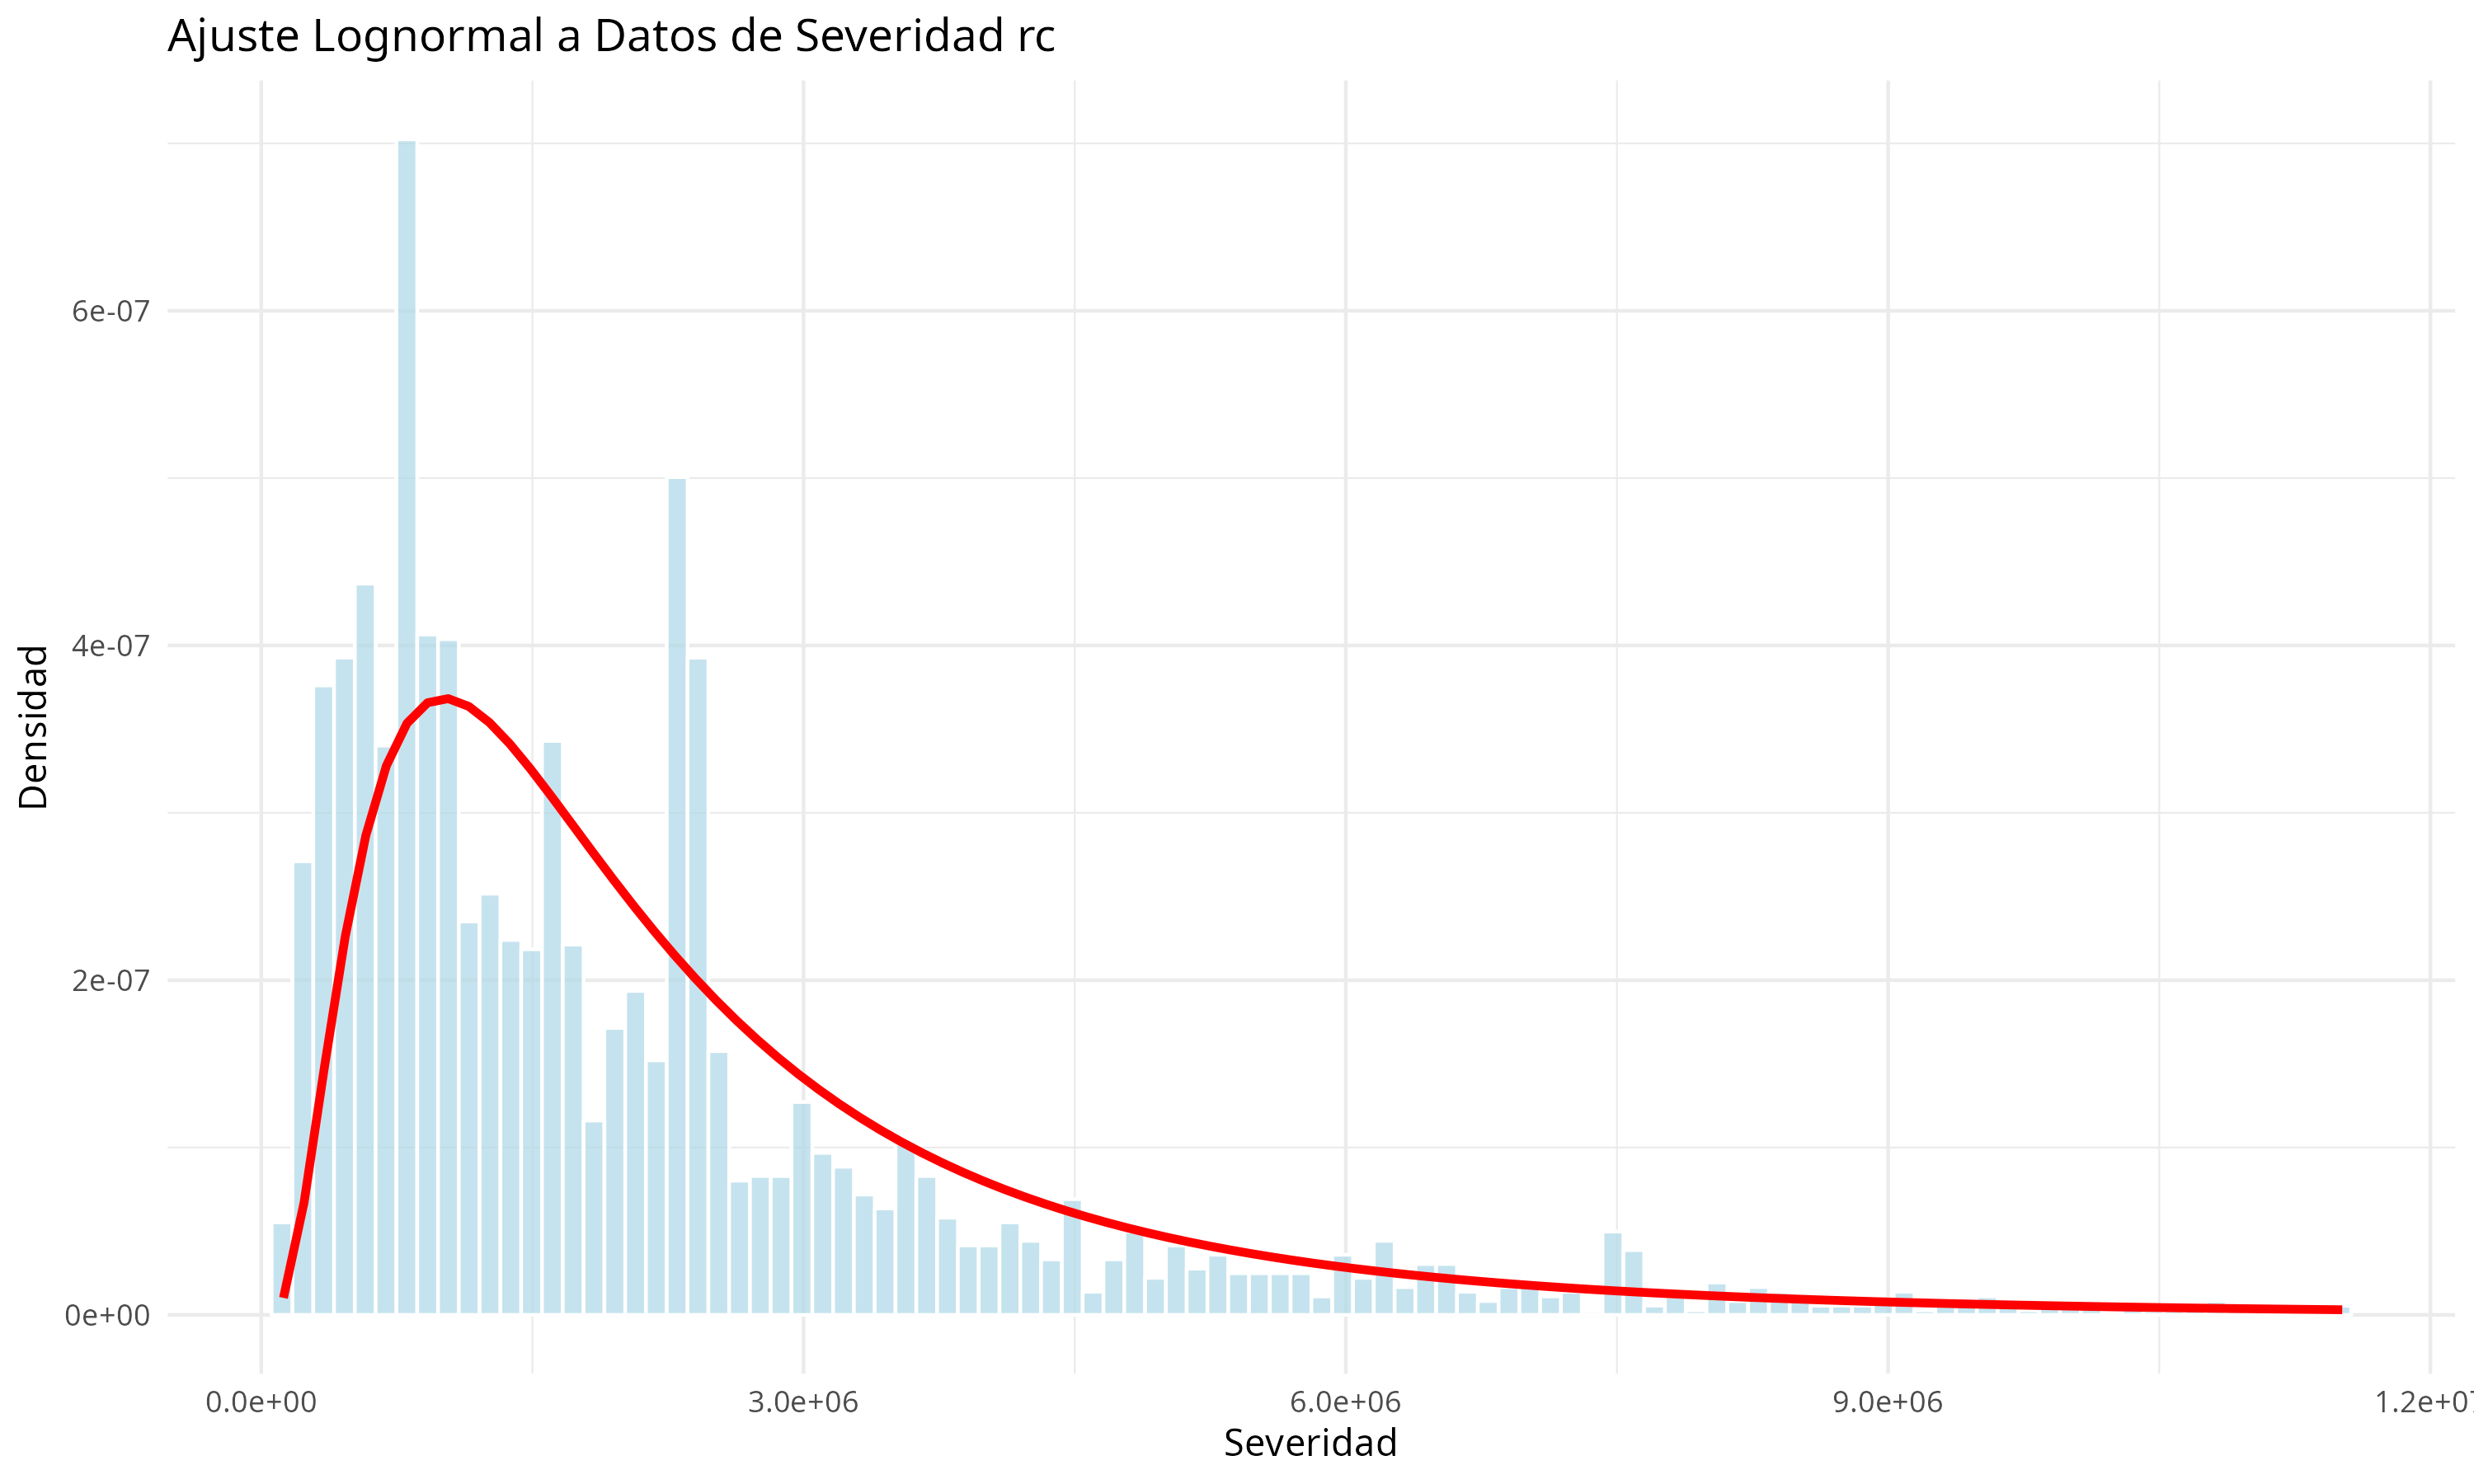
\includegraphics[width=\textwidth]{../images/ajuste_lognormal_rc.png}
        \caption{Ajuste Lognormal RC}
    \end{subfigure}
    \hfill
    \begin{subfigure}{0.45\textwidth}
        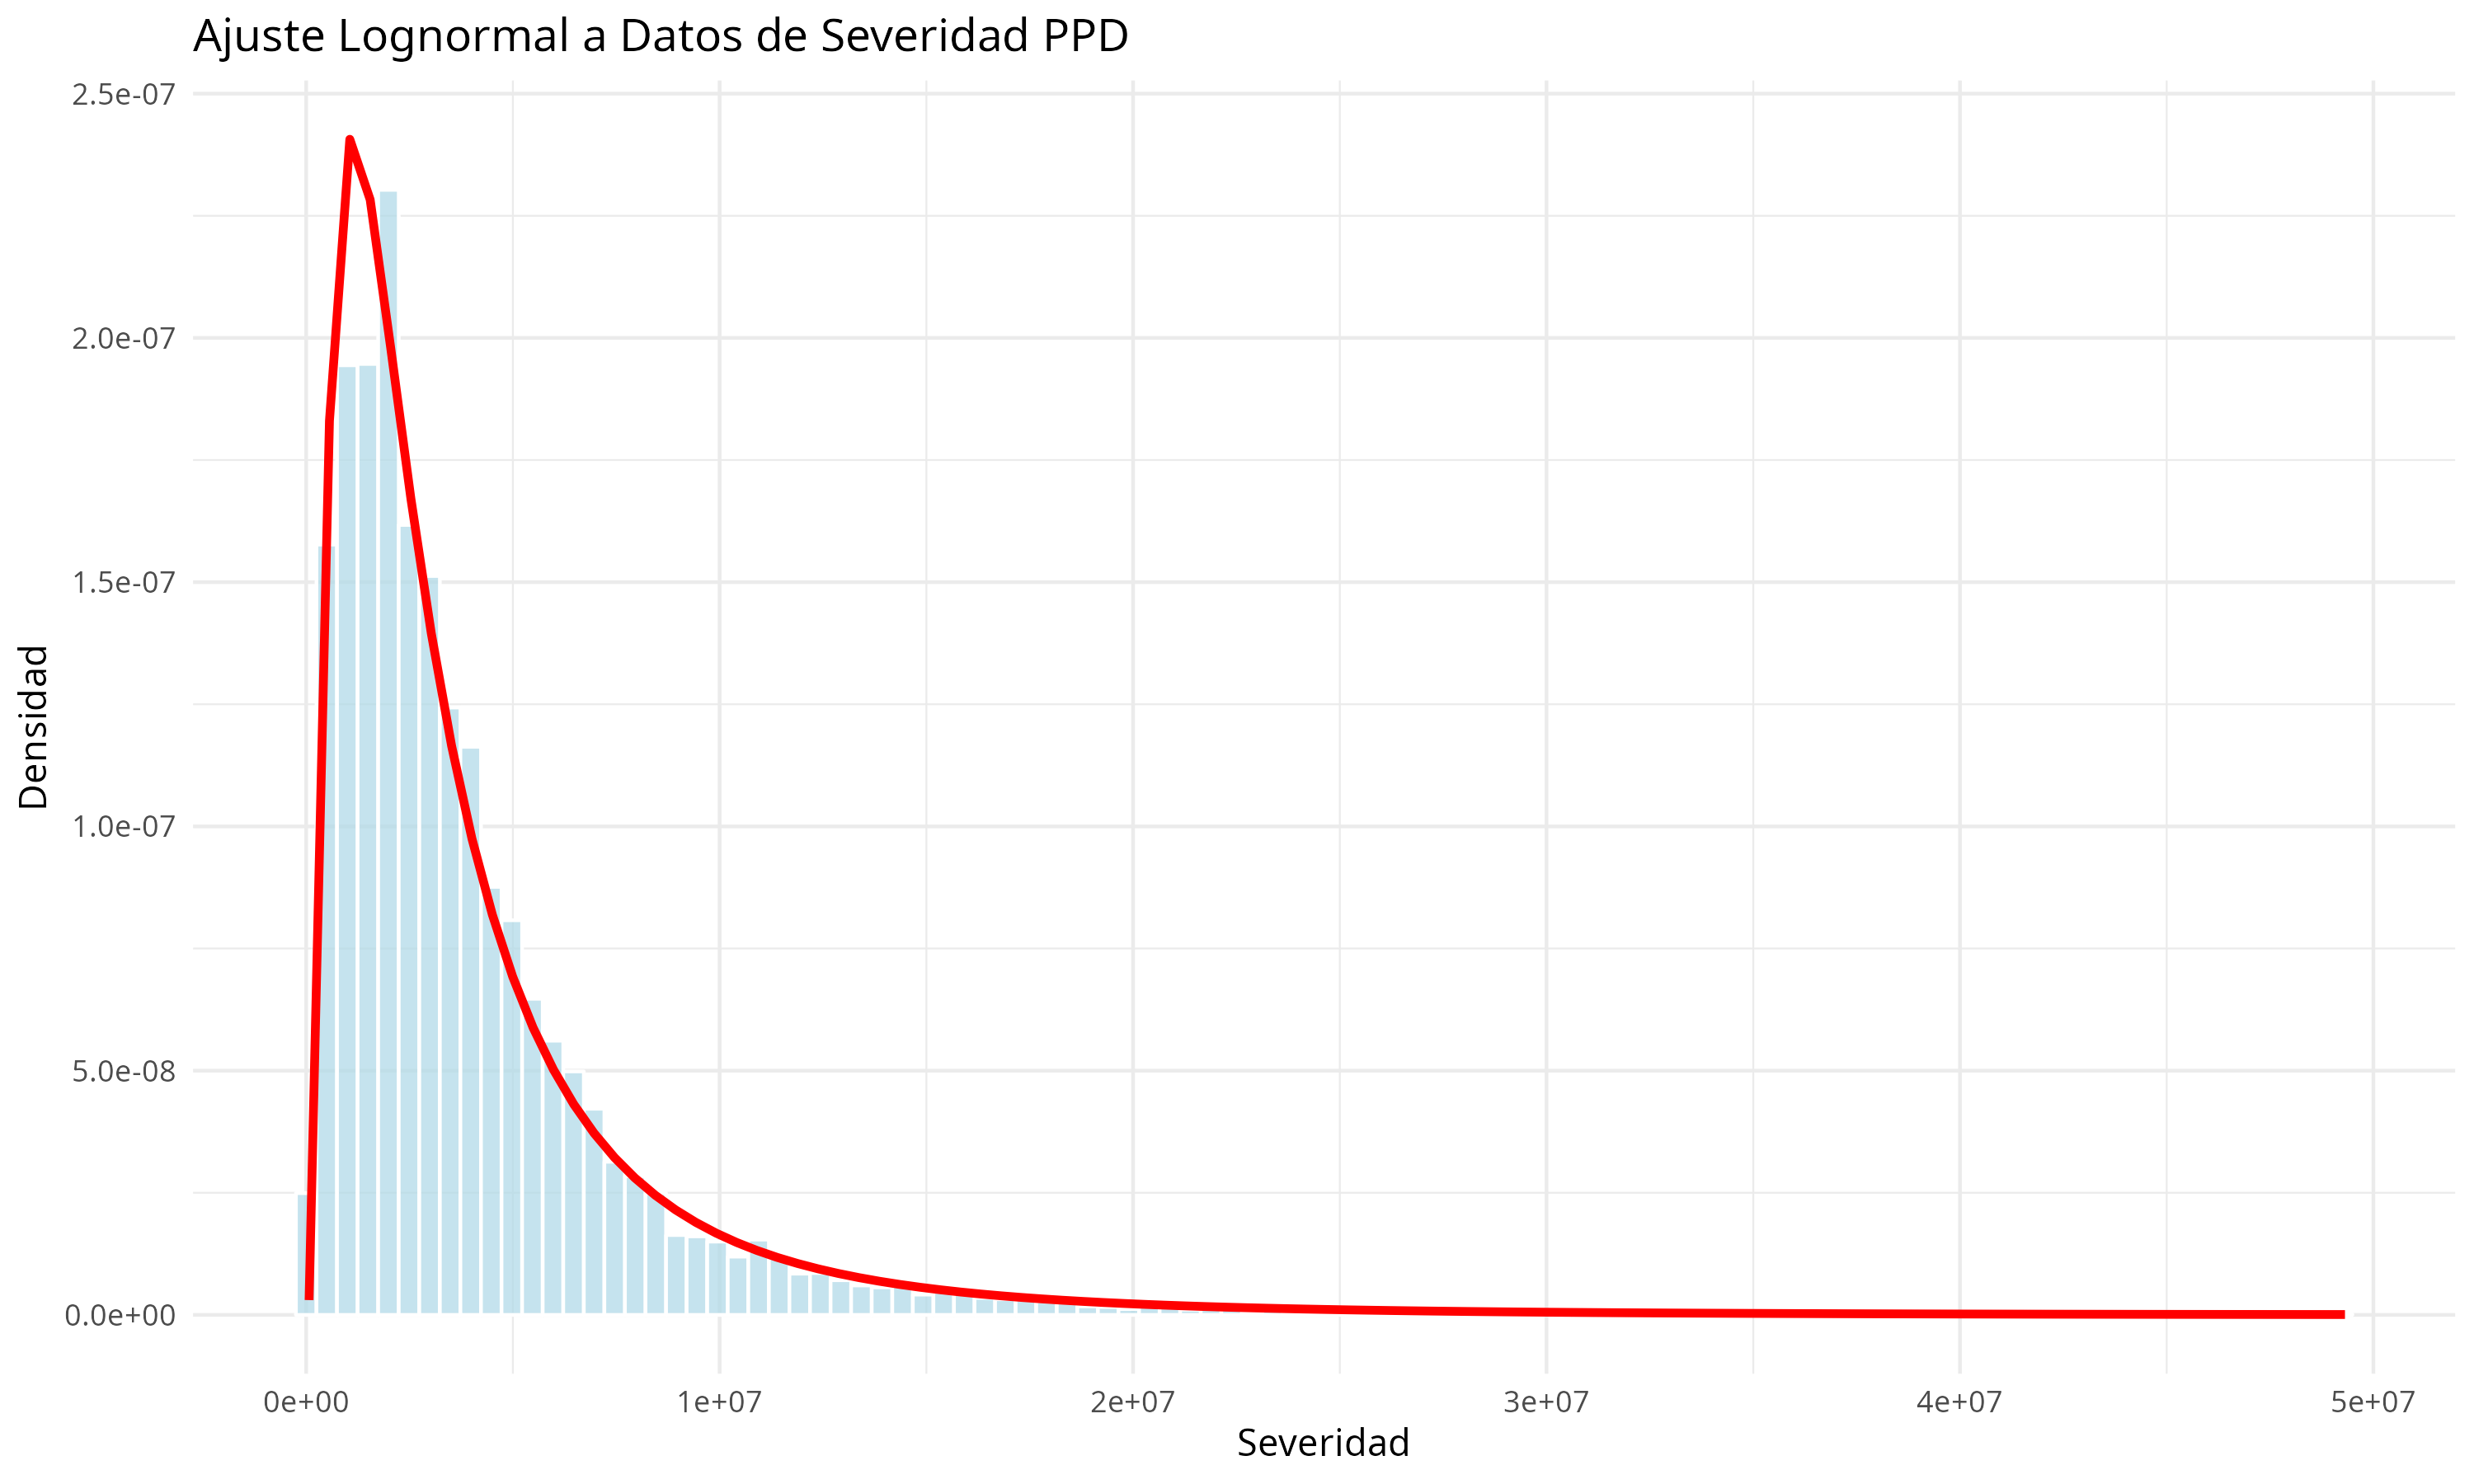
\includegraphics[width=\textwidth]{../images/ajuste_lognormal_pph.png}
        \caption{Ajuste Lognormal PPH}
    \end{subfigure}
\end{figure}

\subsection{Perdidas por cobertura}
a

\subsection{Perdida}
a